\documentclass[12pt]{report}
\usepackage[utf8]{inputenc}
\usepackage[russian]{babel}
%\usepackage[14pt]{extsizes}
\usepackage{listings}
\usepackage{graphicx}
\usepackage{amsmath,amsfonts,amssymb,amsthm,mathtools} 
\usepackage{pgfplots}
\usepackage{filecontents}
\usepackage{float}
\usepackage{indentfirst}
\usepackage{eucal}
\usepackage{enumitem}
%s\documentclass[openany]{book}
\frenchspacing

\usepackage{indentfirst} % Красная строка

\usetikzlibrary{datavisualization}
\usetikzlibrary{datavisualization.formats.functions}

\usepackage{amsmath}


% Для листинга кода:
\lstset{ %
	language=c,                 % выбор языка для подсветки (здесь это С)
	basicstyle=\small\sffamily, % размер и начертание шрифта для подсветки кода
	numbers=left,               % где поставить нумерацию строк (слева\справа)
	numberstyle=\tiny,           % размер шрифта для номеров строк
	stepnumber=1,                   % размер шага между двумя номерами строк
	numbersep=5pt,                % как далеко отстоят номера строк от подсвечиваемого кода
	showspaces=false,            % показывать или нет пробелы специальными отступами
	showstringspaces=false,      % показывать или нет пробелы в строках
	showtabs=false,             % показывать или нет табуляцию в строках
	frame=single,              % рисовать рамку вокруг кода
	tabsize=2,                 % размер табуляции по умолчанию равен 2 пробелам
	captionpos=t,              % позиция заголовка вверху [t] или внизу [b] 
	breaklines=true,           % автоматически переносить строки (да\нет)
	breakatwhitespace=false, % переносить строки только если есть пробел
	escapeinside={\#*}{*)}   % если нужно добавить комментарии в коде
}


\usepackage[left=2cm,right=2cm, top=2cm,bottom=2cm,bindingoffset=0cm]{geometry}
% Для измененных титулов глав:
\usepackage{titlesec, blindtext, color} % подключаем нужные пакеты
\definecolor{gray75}{gray}{0.75} % определяем цвет
\newcommand{\hsp}{\hspace{20pt}} % длина линии в 20pt
% titleformat определяет стиль
\titleformat{\chapter}[hang]{\Huge\bfseries}{\thechapter\hsp\textcolor{gray75}{|}\hsp}{0pt}{\Huge\bfseries}


% plot
\usepackage{pgfplots}
\usepackage{filecontents}
\usetikzlibrary{datavisualization}
\usetikzlibrary{datavisualization.formats.functions}

\begin{document}
	%\def\chaptername{} % убирает "Глава"
	\thispagestyle{empty}
	\begin{titlepage}
		\noindent \begin{minipage}{0.15\textwidth}
			
\includegraphics[width=\linewidth]{b_logo}
		\end{minipage}
		\noindent\begin{minipage}{0.9\textwidth}\centering
			\textbf{Министерство науки и высшего образования Российской Федерации}\\
			\textbf{Федеральное государственное бюджетное образовательное учреждение высшего образования}\\
			\textbf{~~~«Московский государственный технический университет имени Н.Э.~Баумана}\\
			\textbf{(национальный исследовательский университет)»}\\
			\textbf{(МГТУ им. Н.Э.~Баумана)}
		\end{minipage}
		
		\noindent\rule{18cm}{3pt}
		\newline\newline
		\noindent ФАКУЛЬТЕТ $\underline{\text{«Информатика и системы управления»}}$ \newline\newline
		\noindent КАФЕДРА $\underline{\text{«Программное обеспечение ЭВМ и информационные технологии»}}$\newline\newline\newline\newline\newline
		
		\begin{center}
			\noindent\begin{minipage}{1.1\textwidth}\centering
				\Large\textbf{  Отчет по лабораторной работе }\newline
				\textbf{по дисциплине <<Операционные системы>>}\newline
			\end{minipage}
		\end{center}
		
		\noindent\textbf{Тема} $\underline{\text{Системный вызов open~~}}$\newline\newline
		\noindent\textbf{Студент} $\underline{\text{Ляпина Н.В.~~~~~~~~~~~~~~~}}$\newline\newline
		\noindent\textbf{Группа} $\underline{\text{ИУ7-62Б~~~~~~~~~~~~~~~~~~~~~~~}}$\newline\newline
		\noindent\textbf{Оценка (баллы)} $\underline{\text{~~~~~~~~~~~~~~~~~~~~~~}}$\newline\newline
		\noindent\textbf{Преподаватель} $\underline{\text{Рязанова Н.Ю.}}$\newline\newline\newline
		
		\begin{center}
			\vfill
			Москва~---~\the\year
			~г.
		\end{center}
	\end{titlepage}
\setcounter{page}{2}

\section*{Описание структур}

\begin{lstlisting}[label=first,caption=Структура struct filename, language=C]
struct filename {
	const char		*name;	/* pointer to actual string */
	const __user char	*uptr;	/* original userland pointer */
	int			refcnt;
	struct audit_names	*aname;
	const char		iname[];
};
\end{lstlisting}

\begin{lstlisting}[label=first,caption=Структура struct open\_flags, language=C]
struct open_flags {
	int open_flag;
	umode_t mode;
	int acc_mode;
	int intent;
	int lookup_flags;
};
\end{lstlisting}

\begin{lstlisting}[label=first,caption=Структура struct nameidata, language=C]
#define EMBEDDED_LEVELS 2
struct nameidata {
	struct path	path;
	struct qstr	last;
	struct path	root;
	struct inode	*inode; /* path.dentry.d_inode */
	unsigned int	flags, state;
	unsigned	seq, next_seq, m_seq, r_seq;
	int		last_type;
	unsigned	depth;
	int		total_link_count;
	struct saved {
		struct path link;
		struct delayed_call done;
		const char *name;
		unsigned seq;
	} *stack, internal[EMBEDDED_LEVELS];
	struct filename	*name;
	struct nameidata *saved;
	unsigned	root_seq;
	int		dfd;
	vfsuid_t	dir_vfsuid;
	umode_t		dir_mode;
} __randomize_layout;
\end{lstlisting}

\section*{Флаги системного вызова \texttt{open()}}

\texttt{O\_EXEC} --- открыть только для выполнения (результат не определен, при открытии директории).

\texttt{O\_RDONLY} --- открыть только на чтение.

\texttt{O\_RDWR} --- открыть на чтение и запись.

\texttt{O\_SEARCH} --- открыть директорию только для поиска (результат не определен, при использовании с файлами, не являющимися директорией).

\texttt{O\_WRONLY} --- открыть только на запись.

\texttt{O\_APPEND} --- файл открывается в режиме добавления, перед каждой операцией записи файловый указатель будет устанавливаться в конец файла.

\texttt{O\_CLOEXEC} --- включает флаг \texttt{close-on-exec} для нового файлового дескриптора, указание этого флага позволяет программе избегать дополнительных операций fcntl \texttt{F\_SETFD} для установки флага \texttt{FD\_CLOEXEC}.

\texttt{O\_CREAT} --- если файл не существует, то он будет создан.

\texttt{O\_DIRECTORY} --- если файл не является каталогом, то open вернёт ошибку.

\texttt{O\_DSYNC} --- файл открывается в режиме синхронного ввода-вывода (все операции записи для соответствующего дескриптора файла блокируют вызывающий процесс до тех пор, пока данные не будут физически записаны).

\texttt{O\_EXCL} --- если используется совместно с \texttt{O\_CREAT}, то при наличии уже созданного файла вызов завершится ошибкой.

\texttt{O\_NOCTTY} --- если файл указывает на терминальное устройство, то оно не станет терминалом управления процесса, даже при его отсутствии.

\texttt{O\_NOFOLLOW} --- если файл является символической ссылкой, то open вернёт ошибку.

\texttt{O\_NONBLOCK} --- файл открывается, по возможности, в режиме non-blocking, то есть никакие последующие операции над дескриптором файла не заставляют в дальнейшем вызывающий процесс ждать.

\texttt{O\_RSYNC} --- операции записи должны выполняться на том же уровне, что и \texttt{O\_SYNC}.

\texttt{O\_SYNC} --- файл открывается в режиме синхронного ввода-вывода (все операции записи для соответствующего дескриптора файла блокируют вызывающий процесс до тех пор, пока данные не будут физически записаны).

\texttt{O\_TRUNC} --- если файл уже существует, он является обычным файлом и заданный режим позволяет записывать в этот файл, то его длина будет урезана до нуля.

\texttt{O\_LARGEFILE} --- позволяет открывать файлы, размер которых не может быть представлен типом off\_t (long).

\texttt{O\_TMPFILE} --- при наличии данного флага создаётся неименованный временный файл.

\begin{figure}[h!]
            \centering
            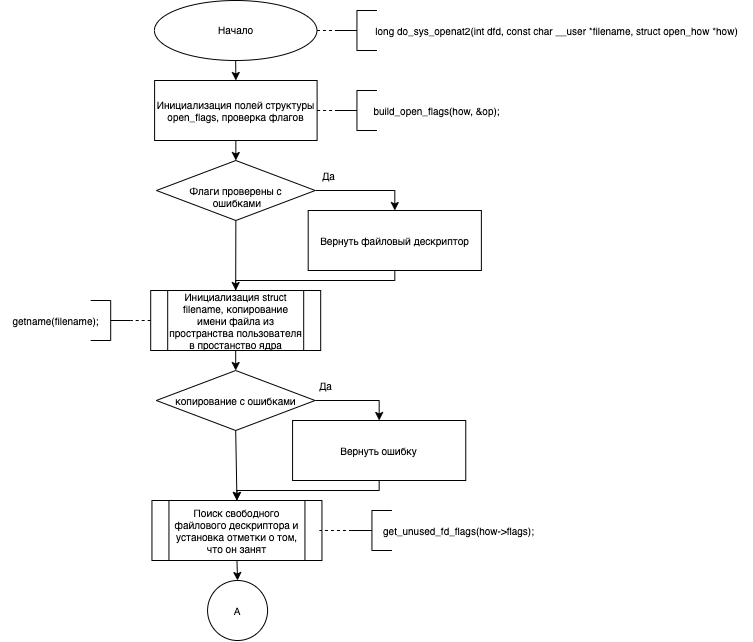
\includegraphics[scale=0.7]{do_sys_open_1.png}
            \caption{Схема алгоритма работы системного вызова do\_sys\_open2. Часть 1}
            \label{png:testing:result}
\end{figure}
\begin{figure}[h!]
            \centering
            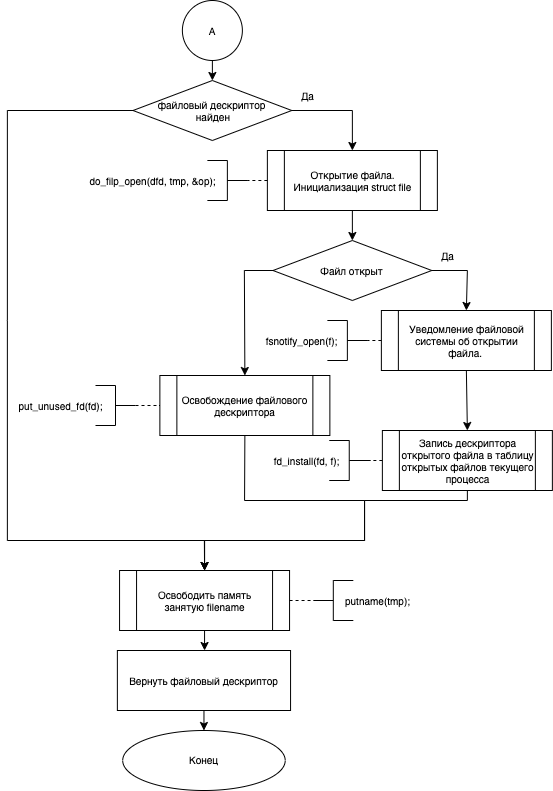
\includegraphics[scale=0.7]{do_sys_open_2.png}
            \caption{Схема алгоритма работы системного вызова do\_sys\_open2. Часть 2}
            \label{png:testing:result}
\end{figure}

\begin{figure}[h!]
	\centering
	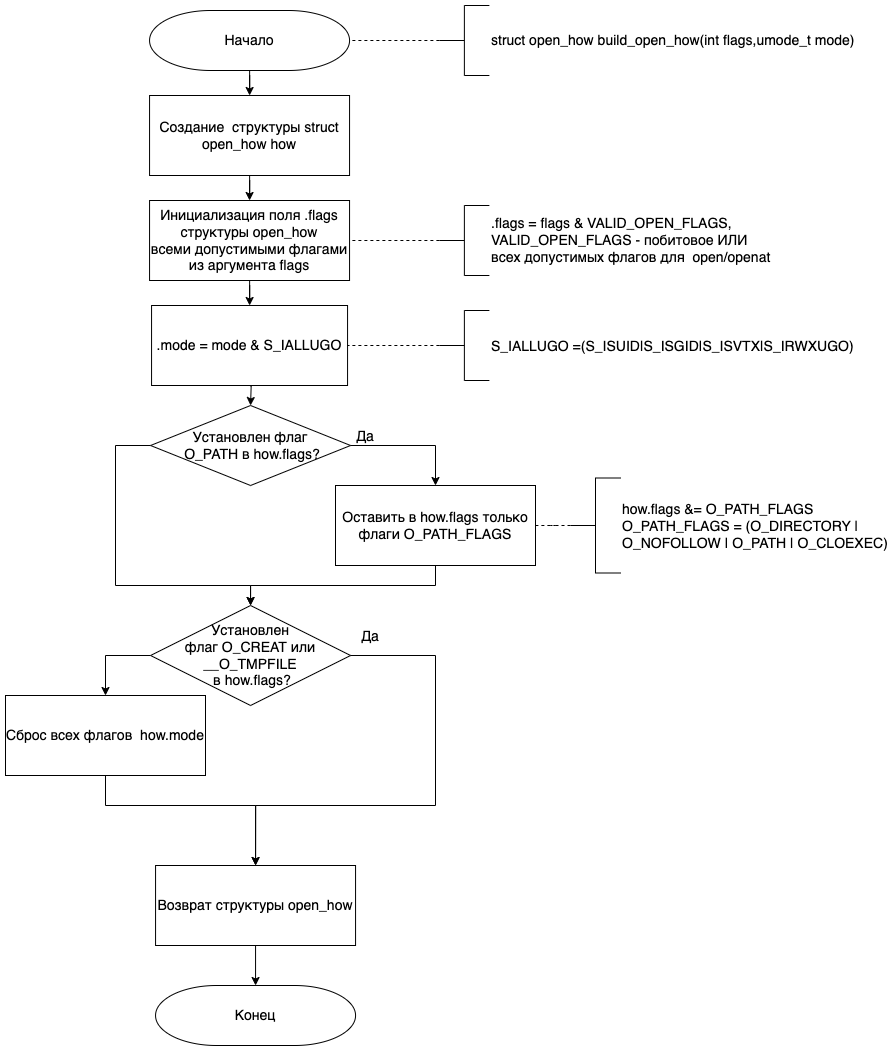
\includegraphics[scale=0.5]{build_open_how.png}
	\caption{Схема алгоритма работы системного вызова build\_open\_how}
	\label{png:testing:result}
\end{figure}

\begin{figure}[h!]
            \centering
            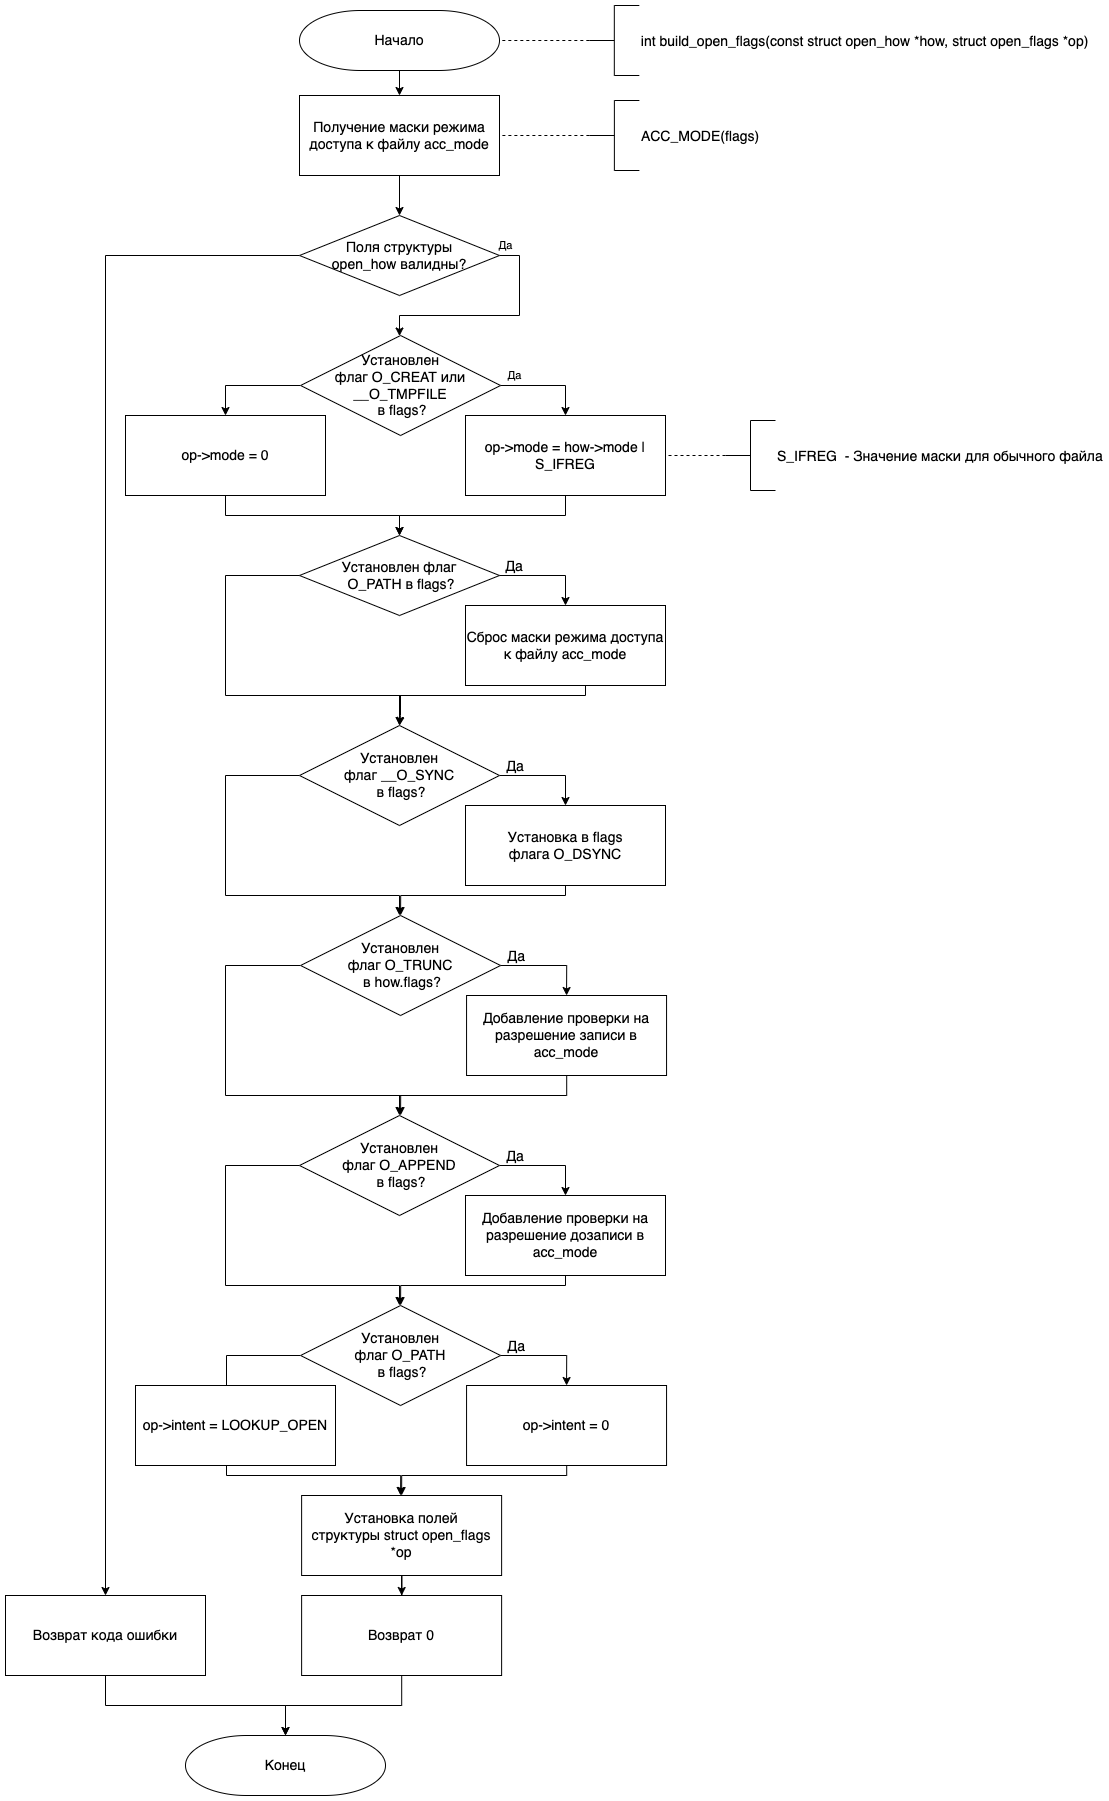
\includegraphics[scale=0.35]{build_open_flags.png}
            \caption{Схема алгоритма работы системного вызова build\_open\_flags}
            \label{png:testing:result}
\end{figure}

\begin{figure}[h!]
            \centering
            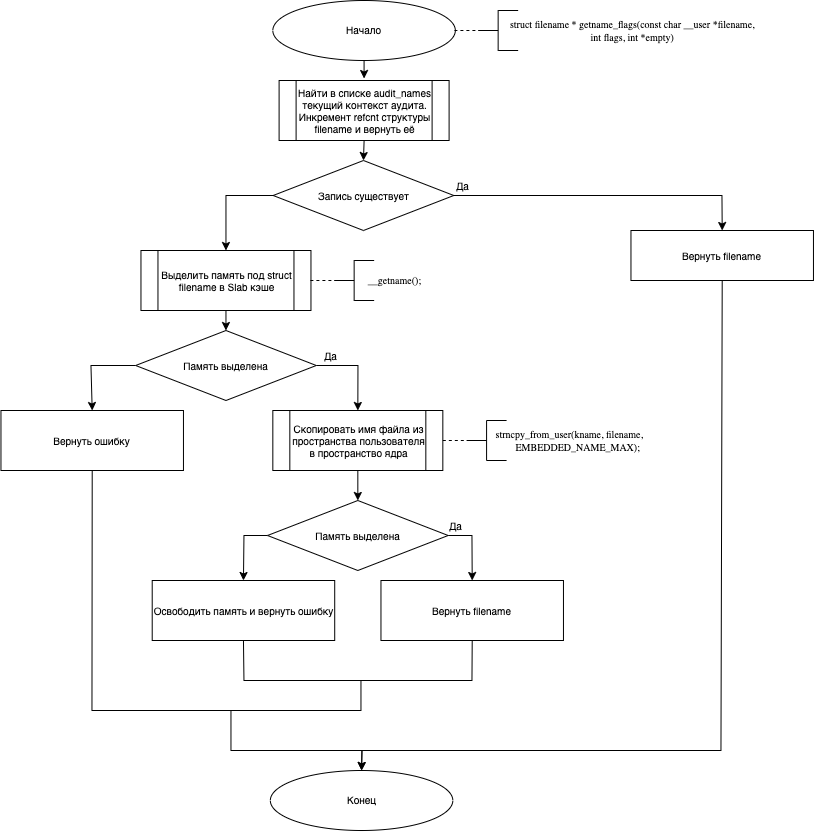
\includegraphics[scale=0.65]{getname_flags.png}
            \caption{Схема алгоритма работы системного вызова getname\_flags}
            \label{png:testing:result}
\end{figure}

\begin{figure}[h!]
            \centering
            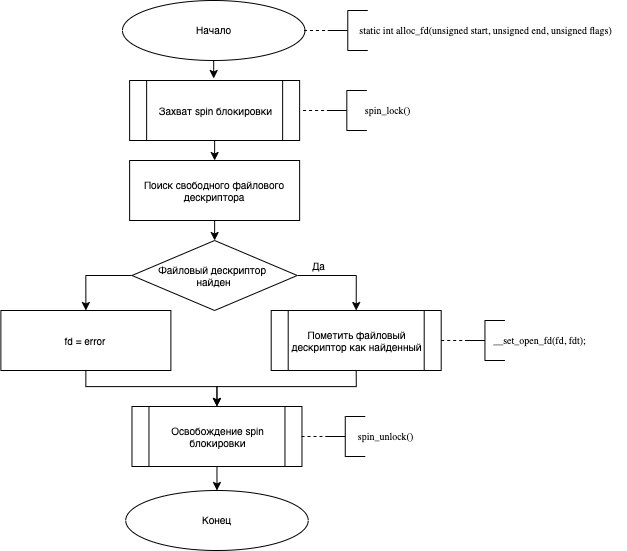
\includegraphics[scale=0.7]{alloc_fd.png}
            \caption{Схема алгоритма работы системного вызова alloc\_fd}
            \label{png:testing:result}
\end{figure}

\begin{figure}[h!]
            \centering
            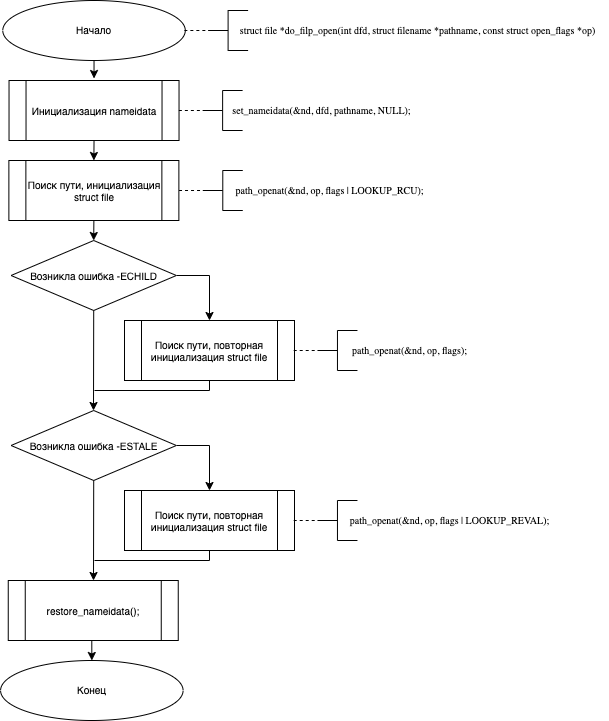
\includegraphics[scale=0.7]{do_filp_open.png}
            \caption{Схема алгоритма работы системного вызова do\_filp\_open}
            \label{png:testing:result}
\end{figure}

\begin{figure}[h!]
            \centering
            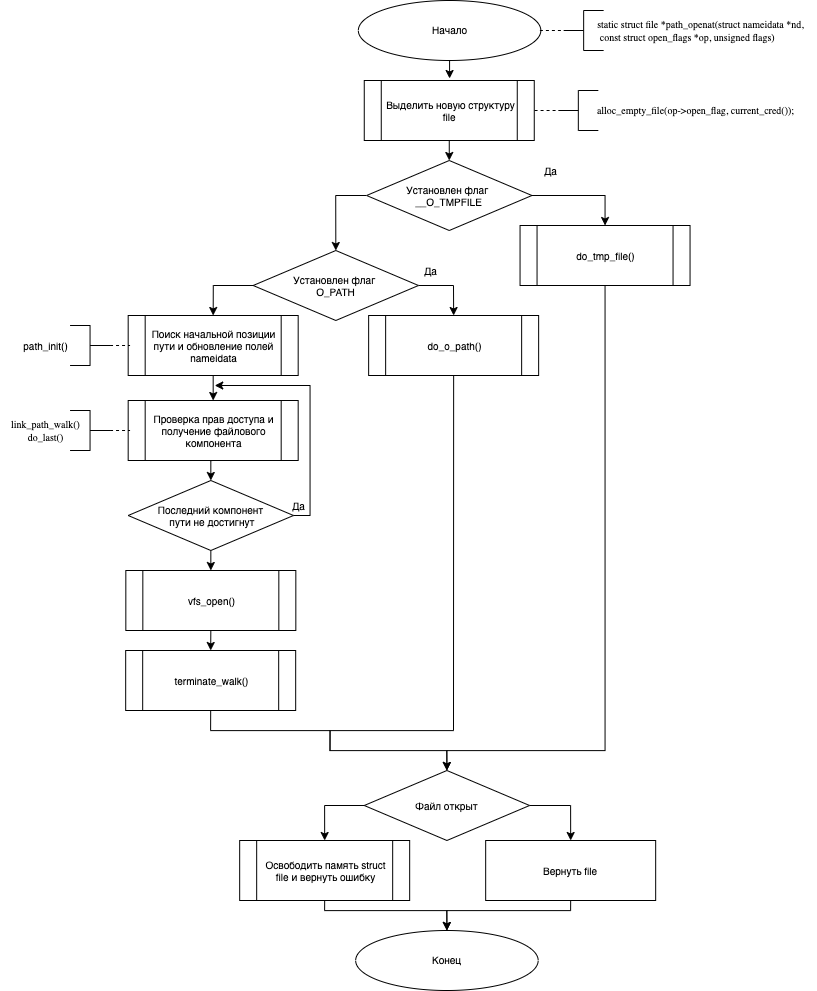
\includegraphics[scale=0.6]{path_openat.png}
            \caption{Схема алгоритма работы системного вызова path\_openat}
            \label{png:testing:result}
\end{figure}

\begin{figure}[h!]
            \centering
            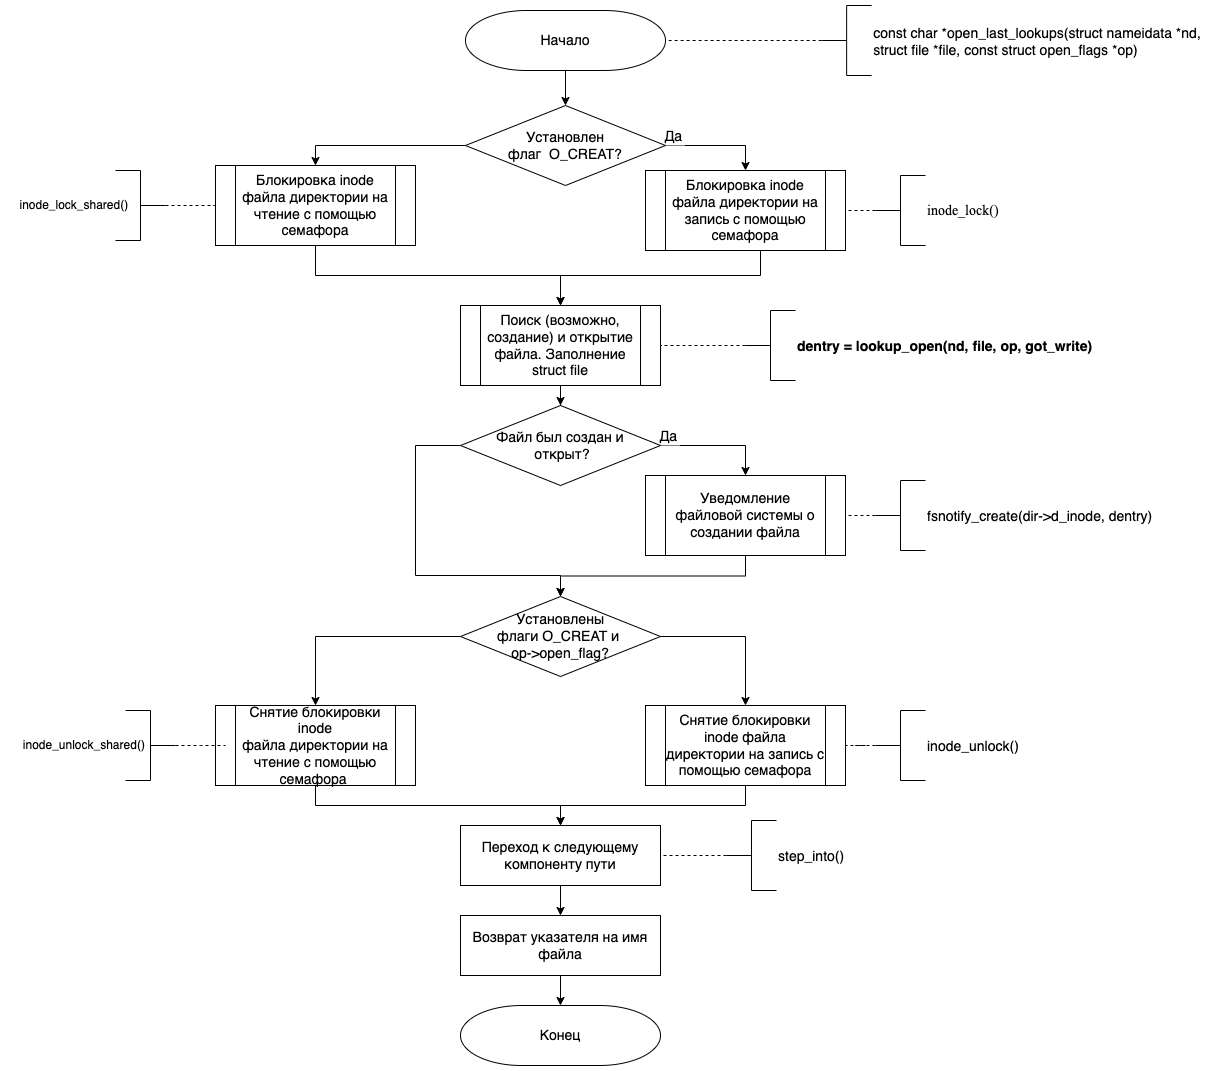
\includegraphics[scale=0.4]{open_last_lookups.png}
            \caption{Схема алгоритма работы системного вызова open\_last\_lookups}
            \label{png:testing:result}
\end{figure}

\begin{figure}[h!]
            \centering
            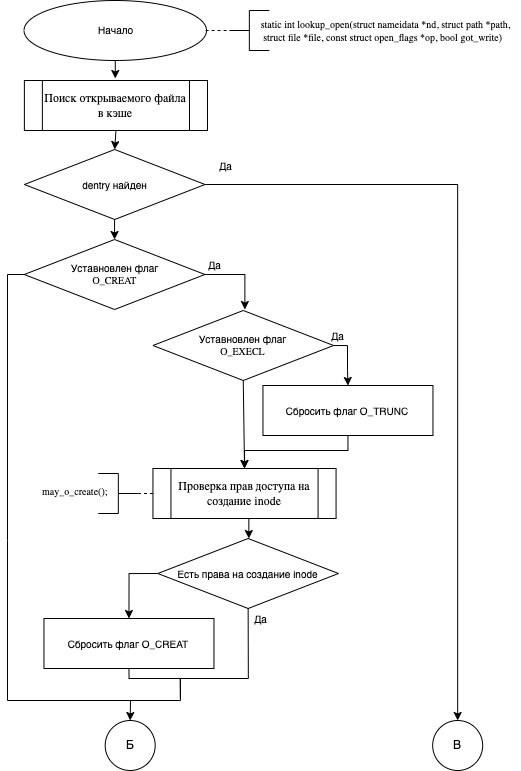
\includegraphics[scale=0.7]{lookups_open1.png}
            \caption{Схема алгоритма работы системного вызова lookup\_open. Часть 1}
            \label{png:testing:result}
\end{figure}

\begin{figure}[h!]
	\centering
	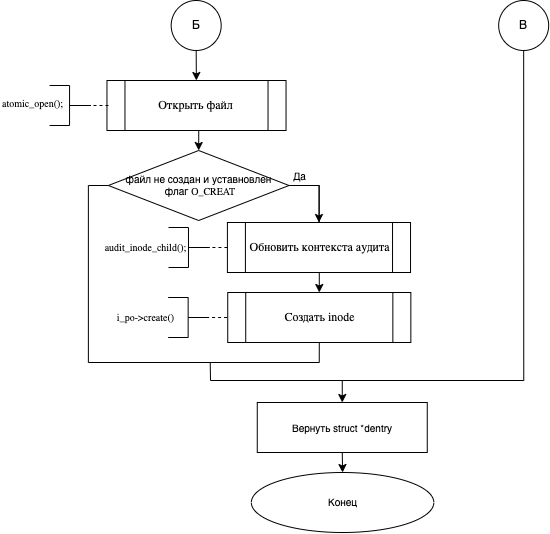
\includegraphics[scale=0.7]{lookups_open2.png}
	\caption{Схема алгоритма работы системного вызова lookup\_open. Часть 2}
	\label{png:testing:result}
\end{figure}

\begin{figure}[h!]
	\centering
	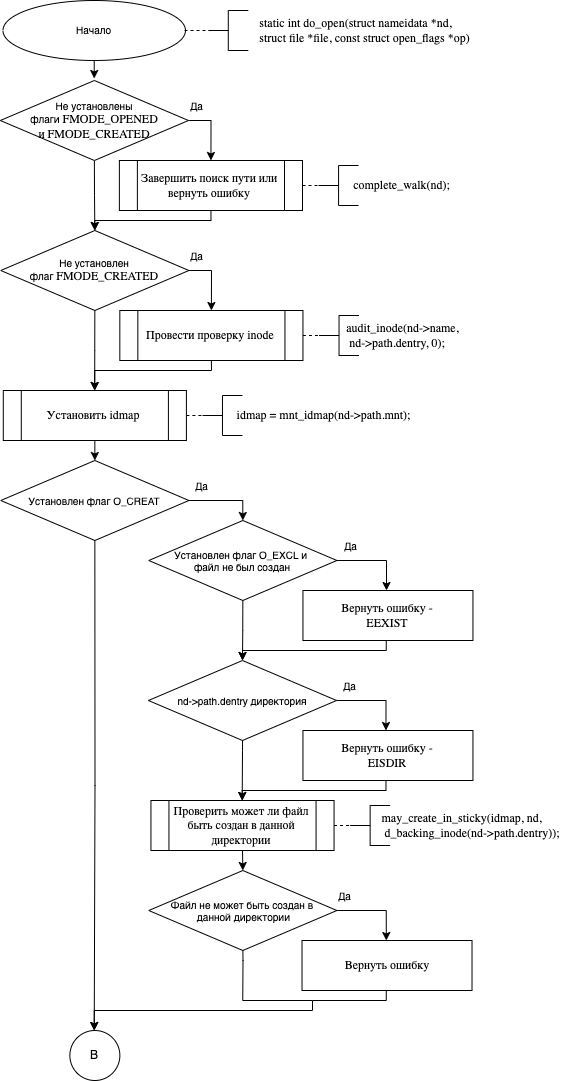
\includegraphics[scale=0.5]{do_open1.png}
	\caption{Схема алгоритма работы системного вызова do\_open. Часть 1}
	\label{png:testing:result}
\end{figure}

\begin{figure}[h!]
	\centering
	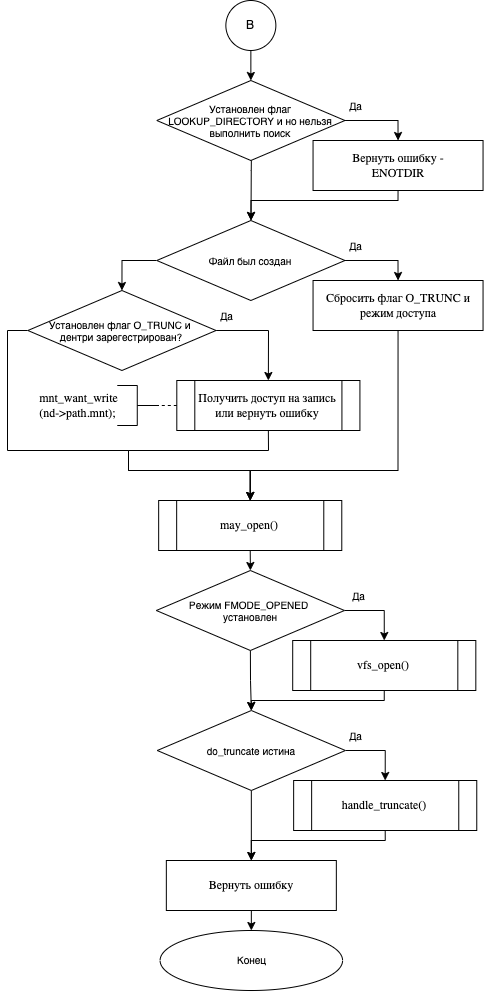
\includegraphics[scale=0.5]{do_open2.png}
	\caption{Схема алгоритма работы системного вызова do\_open. Часть 2}
	\label{png:testing:result}
\end{figure}
\newpage
\end{document}